% Options for packages loaded elsewhere
\PassOptionsToPackage{unicode}{hyperref}
\PassOptionsToPackage{hyphens}{url}
%
\documentclass[
]{article}
\usepackage{amsmath,amssymb}
\usepackage{lmodern}
\usepackage{iftex}
\ifPDFTeX
  \usepackage[T1]{fontenc}
  \usepackage[utf8]{inputenc}
  \usepackage{textcomp} % provide euro and other symbols
\else % if luatex or xetex
  \usepackage{unicode-math}
  \defaultfontfeatures{Scale=MatchLowercase}
  \defaultfontfeatures[\rmfamily]{Ligatures=TeX,Scale=1}
\fi
% Use upquote if available, for straight quotes in verbatim environments
\IfFileExists{upquote.sty}{\usepackage{upquote}}{}
\IfFileExists{microtype.sty}{% use microtype if available
  \usepackage[]{microtype}
  \UseMicrotypeSet[protrusion]{basicmath} % disable protrusion for tt fonts
}{}
\makeatletter
\@ifundefined{KOMAClassName}{% if non-KOMA class
  \IfFileExists{parskip.sty}{%
    \usepackage{parskip}
  }{% else
    \setlength{\parindent}{0pt}
    \setlength{\parskip}{6pt plus 2pt minus 1pt}}
}{% if KOMA class
  \KOMAoptions{parskip=half}}
\makeatother
\usepackage{xcolor}
\usepackage[margin=1in]{geometry}
\usepackage{color}
\usepackage{fancyvrb}
\newcommand{\VerbBar}{|}
\newcommand{\VERB}{\Verb[commandchars=\\\{\}]}
\DefineVerbatimEnvironment{Highlighting}{Verbatim}{commandchars=\\\{\}}
% Add ',fontsize=\small' for more characters per line
\usepackage{framed}
\definecolor{shadecolor}{RGB}{248,248,248}
\newenvironment{Shaded}{\begin{snugshade}}{\end{snugshade}}
\newcommand{\AlertTok}[1]{\textcolor[rgb]{0.94,0.16,0.16}{#1}}
\newcommand{\AnnotationTok}[1]{\textcolor[rgb]{0.56,0.35,0.01}{\textbf{\textit{#1}}}}
\newcommand{\AttributeTok}[1]{\textcolor[rgb]{0.77,0.63,0.00}{#1}}
\newcommand{\BaseNTok}[1]{\textcolor[rgb]{0.00,0.00,0.81}{#1}}
\newcommand{\BuiltInTok}[1]{#1}
\newcommand{\CharTok}[1]{\textcolor[rgb]{0.31,0.60,0.02}{#1}}
\newcommand{\CommentTok}[1]{\textcolor[rgb]{0.56,0.35,0.01}{\textit{#1}}}
\newcommand{\CommentVarTok}[1]{\textcolor[rgb]{0.56,0.35,0.01}{\textbf{\textit{#1}}}}
\newcommand{\ConstantTok}[1]{\textcolor[rgb]{0.00,0.00,0.00}{#1}}
\newcommand{\ControlFlowTok}[1]{\textcolor[rgb]{0.13,0.29,0.53}{\textbf{#1}}}
\newcommand{\DataTypeTok}[1]{\textcolor[rgb]{0.13,0.29,0.53}{#1}}
\newcommand{\DecValTok}[1]{\textcolor[rgb]{0.00,0.00,0.81}{#1}}
\newcommand{\DocumentationTok}[1]{\textcolor[rgb]{0.56,0.35,0.01}{\textbf{\textit{#1}}}}
\newcommand{\ErrorTok}[1]{\textcolor[rgb]{0.64,0.00,0.00}{\textbf{#1}}}
\newcommand{\ExtensionTok}[1]{#1}
\newcommand{\FloatTok}[1]{\textcolor[rgb]{0.00,0.00,0.81}{#1}}
\newcommand{\FunctionTok}[1]{\textcolor[rgb]{0.00,0.00,0.00}{#1}}
\newcommand{\ImportTok}[1]{#1}
\newcommand{\InformationTok}[1]{\textcolor[rgb]{0.56,0.35,0.01}{\textbf{\textit{#1}}}}
\newcommand{\KeywordTok}[1]{\textcolor[rgb]{0.13,0.29,0.53}{\textbf{#1}}}
\newcommand{\NormalTok}[1]{#1}
\newcommand{\OperatorTok}[1]{\textcolor[rgb]{0.81,0.36,0.00}{\textbf{#1}}}
\newcommand{\OtherTok}[1]{\textcolor[rgb]{0.56,0.35,0.01}{#1}}
\newcommand{\PreprocessorTok}[1]{\textcolor[rgb]{0.56,0.35,0.01}{\textit{#1}}}
\newcommand{\RegionMarkerTok}[1]{#1}
\newcommand{\SpecialCharTok}[1]{\textcolor[rgb]{0.00,0.00,0.00}{#1}}
\newcommand{\SpecialStringTok}[1]{\textcolor[rgb]{0.31,0.60,0.02}{#1}}
\newcommand{\StringTok}[1]{\textcolor[rgb]{0.31,0.60,0.02}{#1}}
\newcommand{\VariableTok}[1]{\textcolor[rgb]{0.00,0.00,0.00}{#1}}
\newcommand{\VerbatimStringTok}[1]{\textcolor[rgb]{0.31,0.60,0.02}{#1}}
\newcommand{\WarningTok}[1]{\textcolor[rgb]{0.56,0.35,0.01}{\textbf{\textit{#1}}}}
\usepackage{longtable,booktabs,array}
\usepackage{calc} % for calculating minipage widths
% Correct order of tables after \paragraph or \subparagraph
\usepackage{etoolbox}
\makeatletter
\patchcmd\longtable{\par}{\if@noskipsec\mbox{}\fi\par}{}{}
\makeatother
% Allow footnotes in longtable head/foot
\IfFileExists{footnotehyper.sty}{\usepackage{footnotehyper}}{\usepackage{footnote}}
\makesavenoteenv{longtable}
\usepackage{graphicx}
\makeatletter
\def\maxwidth{\ifdim\Gin@nat@width>\linewidth\linewidth\else\Gin@nat@width\fi}
\def\maxheight{\ifdim\Gin@nat@height>\textheight\textheight\else\Gin@nat@height\fi}
\makeatother
% Scale images if necessary, so that they will not overflow the page
% margins by default, and it is still possible to overwrite the defaults
% using explicit options in \includegraphics[width, height, ...]{}
\setkeys{Gin}{width=\maxwidth,height=\maxheight,keepaspectratio}
% Set default figure placement to htbp
\makeatletter
\def\fps@figure{htbp}
\makeatother
\setlength{\emergencystretch}{3em} % prevent overfull lines
\providecommand{\tightlist}{%
  \setlength{\itemsep}{0pt}\setlength{\parskip}{0pt}}
\setcounter{secnumdepth}{-\maxdimen} % remove section numbering
\ifLuaTeX
  \usepackage{selnolig}  % disable illegal ligatures
\fi
\IfFileExists{bookmark.sty}{\usepackage{bookmark}}{\usepackage{hyperref}}
\IfFileExists{xurl.sty}{\usepackage{xurl}}{} % add URL line breaks if available
\urlstyle{same} % disable monospaced font for URLs
\hypersetup{
  pdftitle={Titolo del progetto},
  pdfauthor={Domenico Plantamura, Eduardo David Lotto, Manuel D'Alterio Grazioli, Gabriele Fugagnoli},
  hidelinks,
  pdfcreator={LaTeX via pandoc}}

\title{Titolo del progetto}
\author{Domenico Plantamura, Eduardo David Lotto, Manuel D'Alterio
Grazioli, Gabriele Fugagnoli}
\date{}

\begin{document}
\maketitle

{
\setcounter{tocdepth}{2}
\tableofcontents
}
\hfill\break

\hypertarget{introduction}{%
\section{Introduction}\label{introduction}}

\hypertarget{objective-of-the-project}{%
\subsection{Objective of the project}\label{objective-of-the-project}}

Our goal is to investigate whether the salaries earned by the NBA
players during the 2023-2024 season are fair in proportion to their
performance during the current year's Regular season. To analyse
performance, we selected several statistics: from the most common such
as points, rebounds, assists to advanced metrics like Usage, Player
Impact Estimated and Winning Shares. The idea is to deep dive into the
relationship between salaries and performance through different models
in order to understand what kind of relationship there is and which
model best fits the data. Finally, we will compare actual salaries with
those predicted by our models to find out which players (according to
the models) are the most overpaid or underpaid.

\hypertarget{steps-followed}{%
\subsection{Steps followed}\label{steps-followed}}

To perform our analysis we followed these steps:

\begin{enumerate}
\def\labelenumi{\arabic{enumi}.}
\item
  Data collection;
\item
  Data exploration;
\item
  Analysis;
\item
  Interpretation.
\end{enumerate}

We now explain in depth each step.

\hfill\break

\hypertarget{data-collection}{%
\subsection{Data collection}\label{data-collection}}

We performed a web scraping operation from the
\href{https://www.nba.com/stats}{Official NBA Stats} website, from which
we collected most of the stats. Additionally, we downloaded data about
the salaries from \href{https://hoopshype.com/}{Hoopshype} and other
stats of interest from
\href{https://www.basketball-reference.com}{Basketball reference}. All
data concerns the 2023-2024 NBA Regular Season.

\hypertarget{why-consider-only-regular-season-data}{%
\subsubsection{Why consider only Regular Season
data?}\label{why-consider-only-regular-season-data}}

Considering only data about Regular Season without considering players
performance during playoffs limits a bit the potential of our analysis.
On one hand, it's reasonable to infer that player performance during
playoffs should have an important weight in determining his salary. On
the other hand, considering playoffs in the analysis carries different
issues.

There are teams (and consequently players) that go further than others:
14 out of 30 teams can't qualify for the playoffs. For the teams which
qualify, playoff stats are calculated on a number of games that could
differ greatly between different teams (e.g.~if a team loses in the
first round, it plays from 4 to 7 games. If a team reaches the finals,
it plays from 16 to 28 games). During Regular Season every team plays a
fixed number of games, 82.

Additionally, coaches usually rotate players at their disposal in a
different way during playoffs: for instance, during regular season
approximately 10-12 players for each team take part in the game; during
playoffs it is not uncommon to observe only 7-8 players that come into
play for each team. Furthermore, usually in a playoff game the best
players are more involved compared to Regular season games. It means
that, first of all, they play several more minutes. Moreover, they have
the ball in their hands for a lot of time and consequently their stats
grow a lot; hence, it could happen that few players record a large part
of the entire team's statistics. Considering this, including playoffs
data in the analysis could lead to an overestimation of performance of
2-3 players and to an underestimation of the performance of the rest of
the team.

All in all, it is undeniable that playoffs are a fundamental part of the
season. It is also obvious that if a player has more responsibilities in
that phase he probably deserves a higher salary. But we think that for
the purposes of our analysis, the addition of statistics collected on a
small sample of matches, different for practically every team, with
highly polarized data between the various players may lead to biases if
not handled properly.

We think that considering only the regular season, although leading to a
limited analysis, may be sufficient to grasp the main relationships
between salaries and performance.

\hypertarget{glossary}{%
\subsubsection{Glossary}\label{glossary}}

\begin{itemize}
\tightlist
\item
  \textbf{PLAYER NAME}: name of a player;
\item
  \textbf{SALARY}: salary earned by a player for 2023-2024 season
  (collected from \href{https://hoopshype.com/}{Hoopshype});
\item
  \textbf{AGE}: age of a player;
\item
  \textbf{POS}: ``Position'', the playing position of a player.
\end{itemize}

\hypertarget{traditional-stats-collected-from-the-nba-website}{%
\paragraph{\texorpdfstring{Traditional stats (collected from the
\href{https://www.nba.com/?47}{NBA}
website)}{Traditional stats (collected from the NBA website)}}\label{traditional-stats-collected-from-the-nba-website}}

\begin{itemize}
\tightlist
\item
  \textbf{GP}: ``Games played'', the number of games played by a player
  during the 2023-2024 regular season;
\item
  \textbf{FG\_PCT}: ``Field Goal Percentage'', the percentage of field
  goal attempts that a player makes. Formula: (FGM)/(FGA);
\item
  \textbf{FG3\_PCT}: ``3 Points ``Field Goal Percentage'', the
  percentage of 3pt field goal attempts that a player makes;
\item
  \textbf{FT\_PCT}: ``Free throws Percentage'', the percentage of free
  throws attempts that a player makes;
\item
  \textbf{OREB}: ``Offensive Rebounds'', the number of rebounds a player
  or team has collected while they were on offense;
\item
  \textbf{DREB}: ``Defensive Rebounds'', the number of rebounds a player
  or team has collected while they were on defense;
\item
  \textbf{REB}: ``Rebounds'', a rebound occurs when a player recovers
  the ball after a missed shot. This statistic is the number of total
  rebounds a player has collected on either offense or defense;
\item
  \textbf{AST}: ``Assists'', the number of assists (passes that lead
  directly to a made basket) by a player;
\item
  \textbf{TOV}: ``Turnovers'', a turnover occurs when a player on
  offense loses the ball to the defense;
\item
  \textbf{STL}: ``Steals'', number of times a defensive player takes the
  ball from a player on offense, causing a turnover;
\item
  \textbf{BLK}: ``Blocks'', a block occurs when an offensive player
  attempts a shot, and the defense player tips the ball, blocking their
  chance to score;
\item
  \textbf{BLKA}: ``Blocks Against'', The number of shots attempted by a
  player or team that are blocked by a defender
\item
  \textbf{PF}: ``Personal fouls'', the number of personal fouls a player
  or team committed;
\item
  \textbf{PFD}: ``Personal fouls drawn'', the number of personal fouls
  that are drawn by a player or team;
\item
  \textbf{PTS}: ``Points'', the number of points scored by a player;
\item
  \textbf{MIN}: ``Minutes played'', number of minutes played by a player
  during the 2023-2024 Regular season;
\item
  \textbf{MIN\_G}: ``Minutes played per game''.
\end{itemize}

\hypertarget{advanced-stats-collected-from-the-nba-website}{%
\paragraph{\texorpdfstring{Advanced stats (collected from the
\href{https://www.nba.com/?47}{NBA}
website)}{Advanced stats (collected from the NBA website)}}\label{advanced-stats-collected-from-the-nba-website}}

\begin{itemize}
\tightlist
\item
  \textbf{OFF\_RATING}: ``Offensive Rating'', measures a team's points
  points scored per 100 possessions while a player is on the court.
  Formula: 100*((Points)/(POSS);
\item
  \textbf{DEF\_RATING}: ``Defensive Rating'', the number of points per
  100 possessions that the team allows while a player is on the court.
  Formula: 100*((Opp Points)/(Opp POSS));
\item
  \textbf{NET\_RATING}: ``Net Rating'', Measures a team's point
  differential per 100 possessions while a player is on the court.
  Formula: OFFRTG - DEFRTG;
\item
  \textbf{AST\_TO}: ``Assist to Turnover Ratio'', the number of assists
  for a player compared to the number of turnovers committed;
\item
  \textbf{TS\_PCT}: ``True Shooting Percentage'', a shooting percentage
  that factors in the value of three-point field goals and free throws
  in addition to conventional two-point field goals. Formula: Points/
  {[}2\emph{(Field Goals Attempted+0.44}Free Throws Attempted){]};
\item
  \textbf{USG\_PCT}: ``Usage Percentage'', the percentage of team plays
  used by a player when they are on the floor. Formula: (FGA +
  Possession Ending FTA + TO) / POSS;
\item
  \textbf{PIE}: ``Player Impact Estimate'', measures a player's overall
  statistical contribution against the total statistics in games they
  play in. PIE yields results which are comparable to other advanced
  statistics (e.g.~PER) using a simple formula. Formula: (PTS + FGM +
  FTM - FGA - FTA + DREB + (.5 * OREB) + AST + STL + (.5 * BLK) - PF -
  TO) / (GmPTS + GmFGM + GmFTM - GmFGA - GmFTA + GmDREB + (.5 * GmOREB)
  + GmAST + GmSTL + (.5 * GmBLK) - GmPF - GmTO).
\end{itemize}

The stats below are collected from
\href{https://www.basketball-reference.com}{Basketball Reference}:

\begin{itemize}
\tightlist
\item
  \textbf{WS}: ``Win Shares'', attempts to divvy up credit for team
  success to the individuals on the team. It is calculated using player,
  team and league-wide statistics and the sum of player win shares on a
  given team will be roughly equal to that team's win total for the
  season (more details on the
  \href{https://www.basketball-reference.com/about/ws.html}{Basketball
  Reference page});
\item
  \textbf{BPM}: ``Box Plus/Minus'', a box score estimate of the points
  per 100 possessions that a player contributed above a league-average
  player, translated to an average team;
\item
  \textbf{VORP}: ``Value Over Replacement Player'', a box score estimate
  of the points per 100 TEAM possessions that a player contributed above
  a replacement-level (-2.0) player, translated to an average team and
  prorated to an 82-game season. Multiply by 2.70 to convert to wins
  over replacement.
\end{itemize}

BPM and VORP are calculated per 100 possessions; MIN and WS are
calculated over the whole regular season, MIN\_G is calculated per game.
The other stats are considered per 48 minutes.

\hypertarget{why-statistics-per-48-minutes}{%
\subsubsection{Why statistics per 48
minutes?}\label{why-statistics-per-48-minutes}}

Considering most statistics projected over 48 minutes avoids
overestimating performance for players who play, on average, more
minutes in a game. In this way we think that the contribution of each
player is fairly evaluated and not distorted by the minutes played.

\hypertarget{data-integration-and-cleaning}{%
\subsection{Data integration and
cleaning}\label{data-integration-and-cleaning}}

Once we had obtained the tables of interest, we selected from each table
the statistics useful for analysis (those given in the glossary) and
then merged the slices of the various datasets, removing all the players
who played less than 480 minutes during the entire regular season.

\begin{Shaded}
\begin{Highlighting}[]
\NormalTok{data\_trad\_tot }\OtherTok{\textless{}{-}}\NormalTok{ data\_traditional\_tot[data\_traditional\_tot}\SpecialCharTok{$}\NormalTok{MIN }\SpecialCharTok{\textgreater{}} \DecValTok{480}\NormalTok{, ]}

\NormalTok{data\_st }\OtherTok{\textless{}{-}} \FunctionTok{merge}\NormalTok{(data\_salary, data\_traditional\_per48, }\AttributeTok{by =} \StringTok{"PLAYER\_NAME"}\NormalTok{, }\AttributeTok{all =} \ConstantTok{TRUE}\NormalTok{)}
\NormalTok{data\_ast }\OtherTok{\textless{}{-}} \FunctionTok{merge}\NormalTok{(data\_st, data\_advanced, }\AttributeTok{by =} \StringTok{"PLAYER\_NAME"}\NormalTok{, }\AttributeTok{all =} \ConstantTok{TRUE}\NormalTok{)}
\NormalTok{data\_mast }\OtherTok{\textless{}{-}} \FunctionTok{merge}\NormalTok{(data\_ast, data\_miscellaneous, }\AttributeTok{by =} \StringTok{"PLAYER\_NAME"}\NormalTok{, }\AttributeTok{all =} \ConstantTok{TRUE}\NormalTok{)}
\NormalTok{data\_mastt }\OtherTok{\textless{}{-}} \FunctionTok{merge}\NormalTok{(data\_mast, data\_trad\_tot, }\AttributeTok{by =} \StringTok{"PLAYER\_NAME"}\NormalTok{, }\AttributeTok{all =} \ConstantTok{TRUE}\NormalTok{)}
\NormalTok{final\_dataset }\OtherTok{\textless{}{-}} \FunctionTok{merge}\NormalTok{(data\_mastt, data\_vorp, }\AttributeTok{by =} \StringTok{"PLAYER\_NAME"}\NormalTok{, }\AttributeTok{all =} \ConstantTok{TRUE}\NormalTok{)}
\end{Highlighting}
\end{Shaded}

The reason why we selected players with at least 480 minutes played is
that we wanted to avoid considering stats taken on a too small amount of
minutes. After these operation, the final dataset consists of 360 rows
and 31 columns.

At this stage, we cleaned the data following these other steps:

\begin{itemize}
\tightlist
\item
  NA removal;
\item
  Matching players' names;
\item
  Transforming the Salary column into a numeric one;
\item
  Putting the players' name as row names for the dataset and thus
  removing the PLAYER\_NAME column.
\end{itemize}

\hypertarget{data-exploration}{%
\subsection{Data exploration}\label{data-exploration}}

Before studying the data with formal models, we got an overview through
an exploratory data analysis. For the first part of our analysis we used
only numeric variables, so the categorical parameter `Pos', which you
can see on the table below, was removed from the dataset at this stage.

\begin{longtable}[]{@{}lcccccccccc@{}}
\toprule()
& Salary & AGE & GP & FG\_PCT & FG3\_PCT & FT\_PCT & OREB & DREB & REB &
AST \\
\midrule()
\endhead
Aaron Gordon & 22266182 & 28 & 73 & 0.556 & 0.290 & 0.658 & 3.6 & 6.2 &
9.8 & 5.4 \\
Aaron Holiday & 2346614 & 27 & 78 & 0.446 & 0.387 & 0.921 & 0.9 & 3.8 &
4.7 & 5.3 \\
Aaron Nesmith & 5634257 & 24 & 72 & 0.496 & 0.419 & 0.781 & 1.5 & 5.1 &
6.6 & 2.6 \\
Aaron Wiggins & 1836096 & 25 & 78 & 0.562 & 0.492 & 0.789 & 2.3 & 4.9 &
7.3 & 3.4 \\
Al Horford & 10000000 & 37 & 65 & 0.511 & 0.419 & 0.867 & 2.3 & 9.1 &
11.4 & 4.6 \\
\bottomrule()
\end{longtable}

\begin{longtable}[]{@{}lcccccccccc@{}}
\toprule()
& TOV & STL & BLK & BLKA & PF & PTS & OFF\_RATING & DEF\_RATING &
NET\_RATING & AST\_TO \\
\midrule()
\endhead
Aaron Gordon & 2.2 & 1.2 & 0.9 & 1.2 & 3.0 & 21.2 & 119.8 & 111.1 & 8.7
& 2.47 \\
Aaron Holiday & 2.0 & 1.6 & 0.2 & 0.8 & 4.7 & 19.4 & 110.5 & 107.6 & 2.9
& 2.64 \\
Aaron Nesmith & 1.5 & 1.6 & 1.2 & 1.2 & 5.8 & 21.1 & 119.3 & 115.0 & 4.3
& 1.69 \\
Aaron Wiggins & 2.2 & 2.2 & 0.7 & 1.3 & 3.6 & 21.2 & 115.6 & 110.0 & 5.7
& 1.54 \\
Al Horford & 1.3 & 1.0 & 1.7 & 0.3 & 2.6 & 15.5 & 120.9 & 109.5 & 11.4 &
3.50 \\
\bottomrule()
\end{longtable}

\begin{longtable}[]{@{}lcccccccccc@{}}
\toprule()
& TS\_PCT & USG\_PCT & PIE & PFD & MIN & MIN\_G & Pos & WS & BPM &
VORP \\
\midrule()
\endhead
Aaron Gordon & 0.607 & 0.174 & 0.103 & 4.7 & 2296.810 & 31.46315 & PF &
7.1 & 1.3 & 1.9 \\
Aaron Holiday & 0.578 & 0.158 & 0.078 & 2.5 & 1269.297 & 16.27303 & PG &
2.5 & -1.5 & 0.2 \\
Aaron Nesmith & 0.631 & 0.158 & 0.071 & 3.5 & 1994.655 & 27.70354 & SF &
4.1 & -0.5 & 0.8 \\
Aaron Wiggins & 0.664 & 0.163 & 0.096 & 2.3 & 1227.938 & 15.74280 & SG &
3.7 & 0.7 & 0.8 \\
Al Horford & 0.650 & 0.119 & 0.105 & 0.8 & 1739.797 & 26.76610 & C & 6.2
& 3.6 & 2.5 \\
\bottomrule()
\end{longtable}

Firstly, an analysis of the variable Salary that will be the dependent
variable in the models.

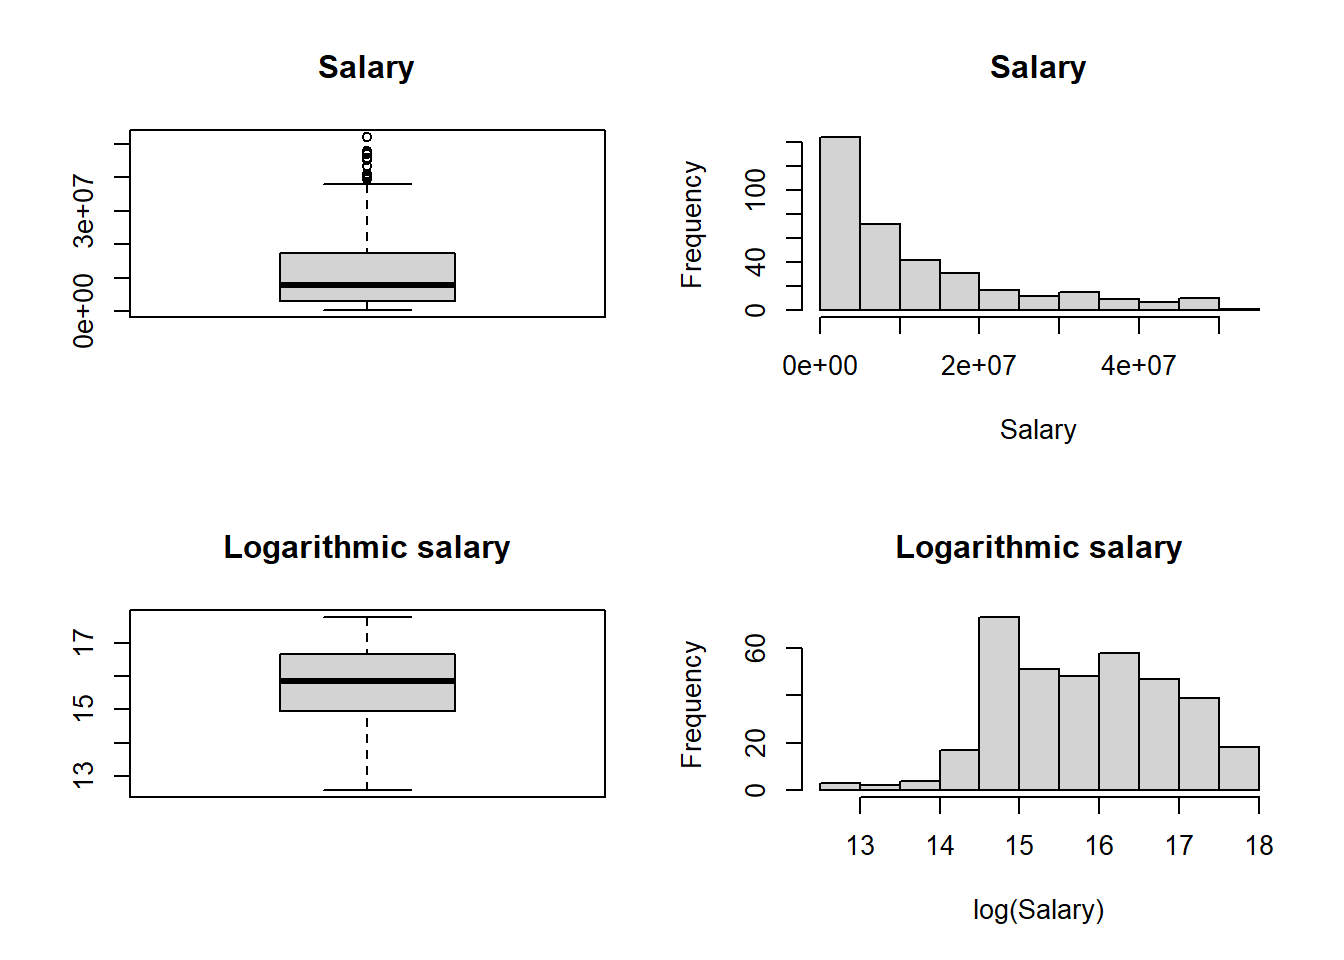
\includegraphics{Report_files/figure-latex/variable-salary-1.pdf}

The boxplot shows that the salary distribution is right skewed, with
some outliers in the right side. We expected this kind of distribution,
the outliers are the players earning the highest salaries. The histogram
also highlights the right skewed distribution. It can be seen that
Salary's log transformation reduces the skewness and makes the
distribution of the variable closer to normal.

In order to study correlations between the predictors of the model, we
used the corrplot function.

\begin{Shaded}
\begin{Highlighting}[]
\FunctionTok{library}\NormalTok{(corrplot)}
\FunctionTok{corrplot}\NormalTok{(}\FunctionTok{cor}\NormalTok{(fd\_numeric), }\AttributeTok{method =} \StringTok{\textquotesingle{}color\textquotesingle{}}\NormalTok{)}
\end{Highlighting}
\end{Shaded}

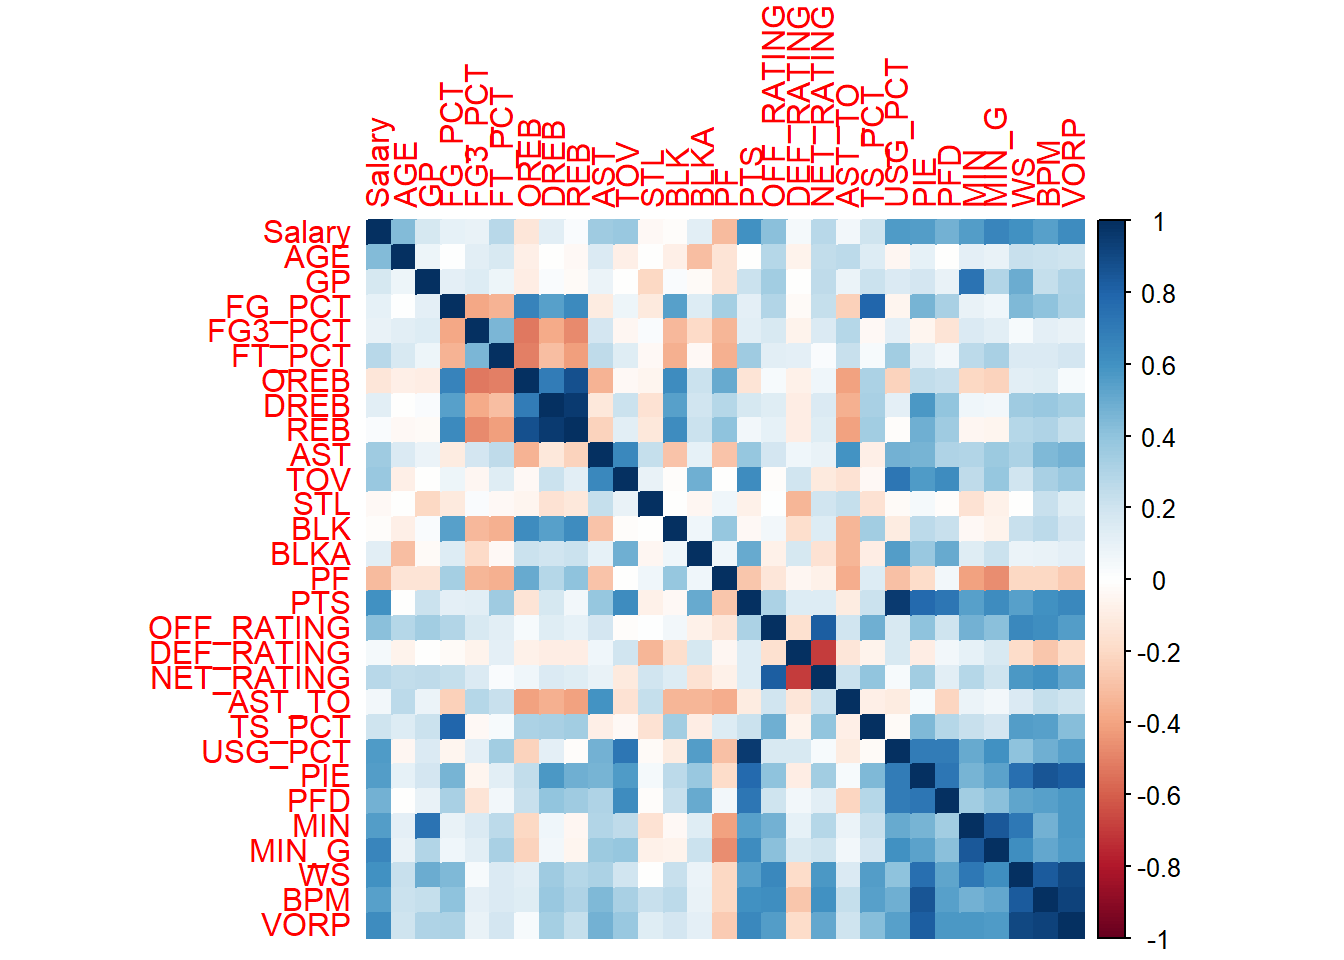
\includegraphics{Report_files/figure-latex/corrplot-independent-variables-1.pdf}

Different correlations between the variables emerge from the corrplot.
With regard to the variable Salary, it is interesting to notice that
Salary is positively correlated with PTS and advanced stats like
USG\_PCT, BPM and VORP: all of these variables are related to players'
shots and point contribution. For what concerns the other variables,
there are some obvious correlations: for instance, between variables MIN
(total minutes played during the regular season) and MIN\_G (minutes
played per game) and between variables REB, OREB and DREB (all related
to rebounds, with the relation REB = OREB + DREB). Additionally, we
expected the positive correlation between BPM and VORP because are both
related to players point estimation. A strong positive correlation
emerges between PTS and USG\_PCT. The usage percentage is ``The
percentage of team plays used by a player when they are on the floor.
Formula: (FGA + Possession Ending FTA + TO) / POSS''. Thus, players with
a high USG\_PCT often make the last play in an offensive possession (a
shot, a free throw or a turnover): it is straightforward that if a
player often ends the offensive possession of his team, he has more
opportunities to score points. For what concerns the negative
correlations, the most interesting are the ones between rebounds
variables (OREB, DREB, REB), FT\_PCT and FG3\_PCT. Players that grab a
lot of rebounds are usually the tallest ones and these players are not
great free throws shooters or 3 point shooters (on average).

\hypertarget{models}{%
\subsection{Models}\label{models}}

We started creating a linear regression model in order to predict
salaries.

\begin{verbatim}
## 
## Call:
## lm(formula = Salary ~ +., data = fd_numeric)
## 
## Residuals:
##       Min        1Q    Median        3Q       Max 
## -18450260  -4028989    276645   4003025  20712902 
## 
## Coefficients:
##               Estimate Std. Error t value Pr(>|t|)    
## (Intercept)  -12550803   28966256  -0.433   0.6651    
## AGE            1057586      93293  11.336   <2e-16 ***
## GP              -21024     118116  -0.178   0.8588    
## FG_PCT        35836089   19086013   1.878   0.0613 .  
## FG3_PCT         -56045    4195524  -0.013   0.9893    
## FT_PCT          975535    6135667   0.159   0.8738    
## OREB           4054377    6865112   0.591   0.5552    
## DREB           4473997    6846450   0.653   0.5139    
## REB           -4315225    6838752  -0.631   0.5285    
## AST             -98527     667680  -0.148   0.8828    
## TOV            2003183    1516145   1.321   0.1873    
## STL             -69046     985541  -0.070   0.9442    
## BLK             601287     664109   0.905   0.3659    
## BLKA          -2253383    1230646  -1.831   0.0680 .  
## PF             -616626     640191  -0.963   0.3362    
## PTS            1117890     623630   1.793   0.0740 .  
## OFF_RATING    16646653    6955245   2.393   0.0172 *  
## DEF_RATING   -16681974    6953008  -2.399   0.0170 *  
## NET_RATING   -16610236    6957987  -2.387   0.0175 *  
## AST_TO         -252115     978605  -0.258   0.7969    
## TS_PCT       -63710004   30332753  -2.100   0.0365 *  
## USG_PCT      -40539821   73391644  -0.552   0.5811    
## PIE         -131534170  115933751  -1.135   0.2574    
## PFD             101829     397847   0.256   0.7981    
## MIN              -4774       4689  -1.018   0.3094    
## MIN_G           696311     299872   2.322   0.0208 *  
## WS             1845668     740418   2.493   0.0132 *  
## BPM            -391702     764769  -0.512   0.6089    
## VORP            663105    1436430   0.462   0.6446    
## ---
## Signif. codes:  0 '***' 0.001 '**' 0.01 '*' 0.05 '.' 0.1 ' ' 1
## 
## Residual standard error: 6712000 on 331 degrees of freedom
## Multiple R-squared:  0.7081, Adjusted R-squared:  0.6834 
## F-statistic: 28.67 on 28 and 331 DF,  p-value: < 2.2e-16
\end{verbatim}

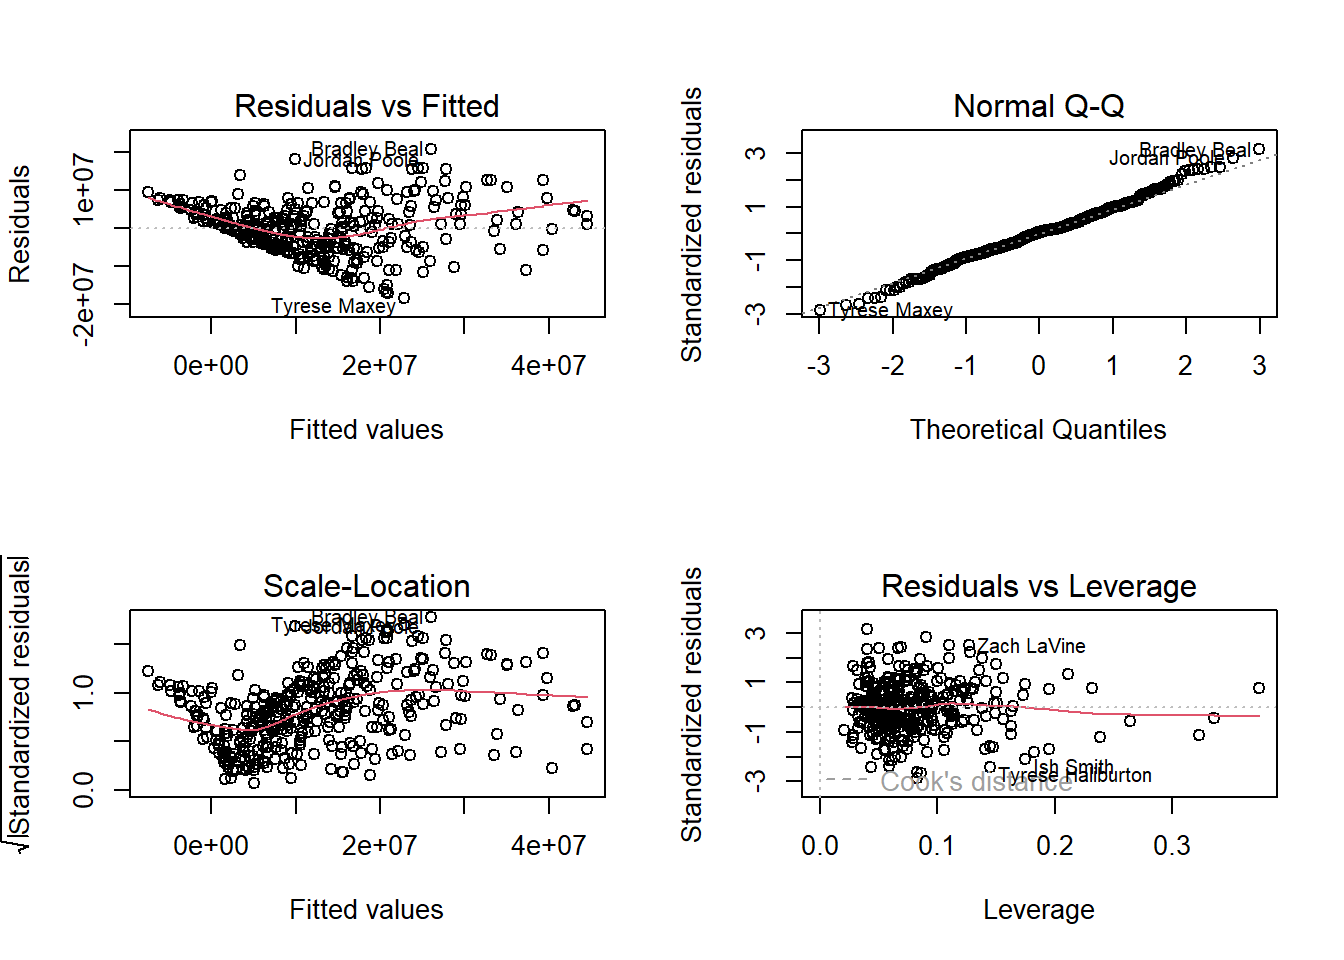
\includegraphics{Report_files/figure-latex/linear-regression-model-1.pdf}

\begin{verbatim}
## [1] 4.142347e+13
\end{verbatim}

The complete model has a good adjusted R-squared of 0.68 and a MSE of
4.14e+13. It emerges that many variables are not significative in
determining the response. Through the residual analysis it is noticeable
that the relationship between fitted values and residuals is not exactly
linear (1st graph). Additionally, in the third graph the points are not
are included in a band of constant amplitude parallel to the x-axis,
hence the omoschedasticity assumption can be doubted.

\begin{verbatim}
## 
## Call:
## lm(formula = log(Salary) ~ +., data = fd_numeric)
## 
## Residuals:
##      Min       1Q   Median       3Q      Max 
## -2.75872 -0.32207  0.02064  0.42623  1.62364 
## 
## Coefficients:
##               Estimate Std. Error t value Pr(>|t|)    
## (Intercept)  1.258e+01  2.744e+00   4.583 6.49e-06 ***
## AGE          9.669e-02  8.838e-03  10.940  < 2e-16 ***
## GP          -5.087e-04  1.119e-02  -0.045   0.9638    
## FG_PCT       3.669e+00  1.808e+00   2.029   0.0432 *  
## FG3_PCT     -7.625e-02  3.975e-01  -0.192   0.8480    
## FT_PCT      -1.574e-01  5.813e-01  -0.271   0.7867    
## OREB         3.180e-01  6.504e-01   0.489   0.6252    
## DREB         4.105e-01  6.486e-01   0.633   0.5273    
## REB         -3.435e-01  6.479e-01  -0.530   0.5963    
## AST          3.954e-02  6.325e-02   0.625   0.5323    
## TOV          1.536e-03  1.436e-01   0.011   0.9915    
## STL          5.077e-02  9.337e-02   0.544   0.5870    
## BLK          7.242e-02  6.291e-02   1.151   0.2505    
## BLKA        -1.802e-01  1.166e-01  -1.545   0.1232    
## PF          -5.294e-02  6.065e-02  -0.873   0.3834    
## PTS          9.972e-02  5.908e-02   1.688   0.0924 .  
## OFF_RATING   1.508e+00  6.589e-01   2.289   0.0227 *  
## DEF_RATING  -1.499e+00  6.587e-01  -2.276   0.0235 *  
## NET_RATING  -1.504e+00  6.592e-01  -2.282   0.0231 *  
## AST_TO      -4.552e-02  9.271e-02  -0.491   0.6237    
## TS_PCT      -6.498e+00  2.874e+00  -2.261   0.0244 *  
## USG_PCT     -2.881e+00  6.953e+00  -0.414   0.6789    
## PIE         -1.715e+01  1.098e+01  -1.562   0.1193    
## PFD          3.123e-02  3.769e-02   0.829   0.4079    
## MIN         -5.447e-05  4.442e-04  -0.123   0.9025    
## MIN_G        5.720e-02  2.841e-02   2.014   0.0449 *  
## WS           1.246e-01  7.014e-02   1.777   0.0765 .  
## BPM          5.637e-02  7.245e-02   0.778   0.4371    
## VORP        -1.639e-01  1.361e-01  -1.204   0.2293    
## ---
## Signif. codes:  0 '***' 0.001 '**' 0.01 '*' 0.05 '.' 0.1 ' ' 1
## 
## Residual standard error: 0.6359 on 331 degrees of freedom
## Multiple R-squared:  0.6516, Adjusted R-squared:  0.6222 
## F-statistic: 22.11 on 28 and 331 DF,  p-value: < 2.2e-16
\end{verbatim}

\includegraphics{Report_files/figure-latex/logarithmic-transformation-1.pdf}

\begin{verbatim}
## [1] 4.703165e+13
\end{verbatim}

With a logarithmic transformation of the dependent variable, the model
shows a slightly lower adjusted R-squared (0.62 vs the previous 0.68)
and a slightly higher MSE (4.70e+13 vs the previous 4.14e+13). Applying
a logarithmic transformation to the dependent variable, the first graph
shows a more linear relationship and the third graph allows to infer a
more constant variance in the error terms. In both models many variables
are not significative in determining the response: for this reason, to
avoid a model that is unnecessary complex, we performed a variable
selection. A logarithmic transformation of the dependent variable Salary
will be applied because, although it slightly worsens the performance of
the model, it makes the salaries distribution closer to normal, it
improves the linearity of the model and it reduces residuals
eteroschedasticity.

\hypertarget{variable-selection}{%
\subsubsection{Variable selection}\label{variable-selection}}

We selected a subset of relevant features starting from the predictors
used in the complete model in order to have a simpler model that is
easier to interpret, without redundant variables and less prone to
overfitting. To do so, we used The regsubsets function which performs
best subset selection by identifying the best model that contains a
given number of predictors, where best is quantified using RSS. We set
the function to return results up to the best 28-variables model.

To find the best balance between model simplicity and precision, we
evaluated the number of parameters to be included in the model through
Mallow's Cp, BIC and Adjusted R-squared.

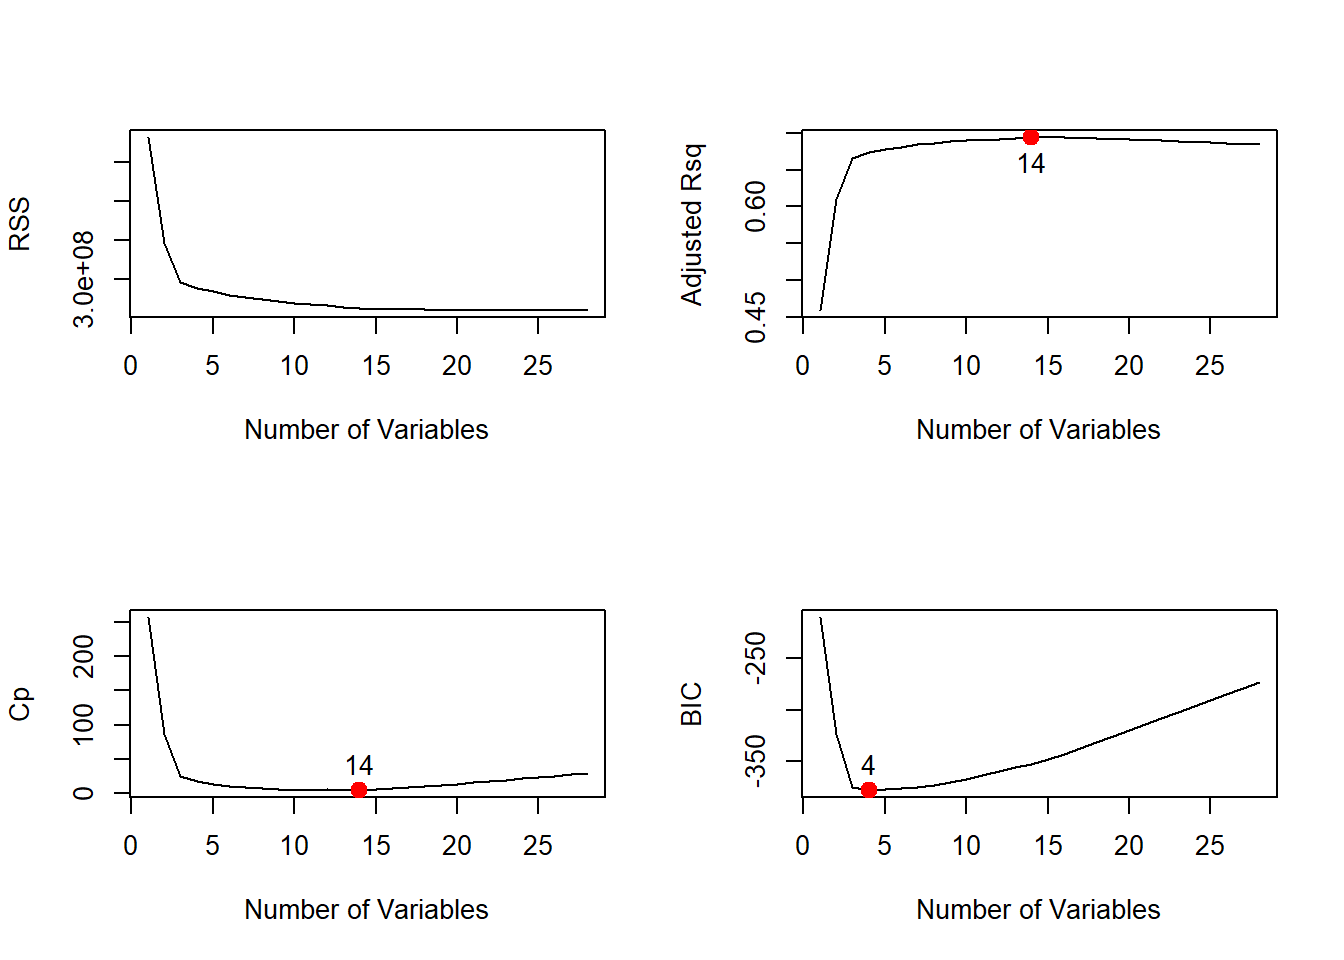
\includegraphics{Report_files/figure-latex/parameters-selection-1.pdf}

Considering Mallow's Cp, the best number of parameters for our model is
12. We obtained the list of parameters from the regsubset function to
get the best model with 12 parameters.

\begin{verbatim}
## 
## Call:
## lm(formula = selected.formula, data = fd_numeric)
## 
## Residuals:
##     Min      1Q  Median      3Q     Max 
## -2.6476 -0.3193  0.0482  0.4315  1.5814 
## 
## Coefficients:
##              Estimate Std. Error t value Pr(>|t|)    
## (Intercept) 10.852025   1.626347   6.673 9.95e-11 ***
## AGE          0.095227   0.008503  11.199  < 2e-16 ***
## FG_PCT       3.445692   1.155704   2.981  0.00307 ** 
## BLK          0.083159   0.049934   1.665  0.09674 .  
## BLKA        -0.167470   0.106759  -1.569  0.11764    
## PTS          0.058816   0.011460   5.132 4.78e-07 ***
## OFF_RATING   1.531106   0.629095   2.434  0.01544 *  
## DEF_RATING  -1.513509   0.629188  -2.405  0.01667 *  
## NET_RATING  -1.520988   0.629121  -2.418  0.01614 *  
## TS_PCT      -5.839664   1.438599  -4.059 6.09e-05 ***
## PIE         -6.258145   2.750650  -2.275  0.02351 *  
## MIN_G        0.059152   0.006890   8.585 3.10e-16 ***
## WS           0.053790   0.026074   2.063  0.03986 *  
## ---
## Signif. codes:  0 '***' 0.001 '**' 0.01 '*' 0.05 '.' 0.1 ' ' 1
## 
## Residual standard error: 0.6263 on 347 degrees of freedom
## Multiple R-squared:  0.6457, Adjusted R-squared:  0.6334 
## F-statistic:  52.7 on 12 and 347 DF,  p-value: < 2.2e-16
\end{verbatim}

The reducted model shows a higher adjusted R-squared, 0.63, compared to
the complete logarithmic model (0.62). It means that, despite the lower
number of variables, this model fits better the data. Different
variables are strongly significant:

\begin{itemize}
\item
  AGE: the positive coefficient associate to the variable show that
  older players earn, on average, more than younger ones. This makes
  sense because the youngest players in the league, rookies(first year
  in NBA) and sophmores(second year in NBA), usually earn less in the
  first years due to particular specifications in their contracts.
\item
  PTS: quite straightforward: positive coefficient means that the
  players who scores more points, on average, have higher salaries.
\item
  TS\_PCT: for what concerns true shooting percentage, the situation is
  peculiar. TS\_PCT weights a player's shooting percentages based on the
  shot type (3-pointer, 2 pointer or free throw). The negative
  coefficient seems counterintuitive, it means that a better TS\_PCT
  reflects, on average, a lower salary. A possible explanation is that
  this metric is high for two players categories: The first category is
  composed by big men which take most of their shots near the basket,
  thus high percentage shots. The second category is composed by 3-point
  shooting specialists, because in the metric the weight for a 3 point
  shoot is higher. The mentioned players are really important into a
  team, but we can say that they often have a limited role: the former
  have to score mostly near the basket, the latter from behind the
  3-point line. Consequently, it makes sense a lower salary for players
  with a limited role. Additionally, shooting percentages are also high
  for players that shoot only few shots in a game; it is reasonable that
  scoring only few shots it's not enough to earn high salaries.
\item
  MIN\_G: players that play on average more minutes in a game earn, on
  average, a higher salary.
\end{itemize}

The variable FG\_PCT is less significative than TS\_PCT, but the
coefficient here is positive. Both the stats measure shooting
percentages, but FG\_PCT does not weight shots and does not consider
free throws. In this way, the previous mentioned effect on 3 point
shooting specialists reduces. It is possible to infer that FG\_PCT
represents better, within this model, the positive impact of good
shooting percentages on wages.

With a level of significance between 0.01 and 0.05 the variables
OFF\_RATING, DEF\_RATING, NET\_RATING, PIE and WS. The positive sign of
OFF\_RATING and WS coefficients and the negative sign of DEF\_RATING
coefficient are in line with what we expected. OFF\_RATING (DEF\_RATING)
represents the points scored (conceded) by the team when the player is
playing, WS measures the player contribution to the team wins. We didn't
expected a negative signs for NET\_RATING (OFF\_RATING - DEF\_RATING)
and PIE, that measures the player impact in the game. For what concerns
PIE, the negative sign has different possible explanations: projecting
PIE per 48 minutes, it is inflated for players who have a high impact on
the game but only for few minutes; It considers a lot of stats, even
stats that seem to be not significative in determining salary; PIE
difference between high salary players and low salary ones is not
proportional to the differences in salaries; it is always difficult
consider defensive contribution with this kind of metrics and it is
reasonable to think that defensive contribution plays an important role
in determining a players salary; PIE does not consider aspects like
leadership and IQ that, like defensive contribution, will certainly have
an impact on the salaries. Anyway, beyond all the possible explanations,
these unexpected negative signs likely depend from other variables not
included in the model.

\hypertarget{correlation-between-dependent-variables}{%
\paragraph{Correlation between dependent
variables}\label{correlation-between-dependent-variables}}

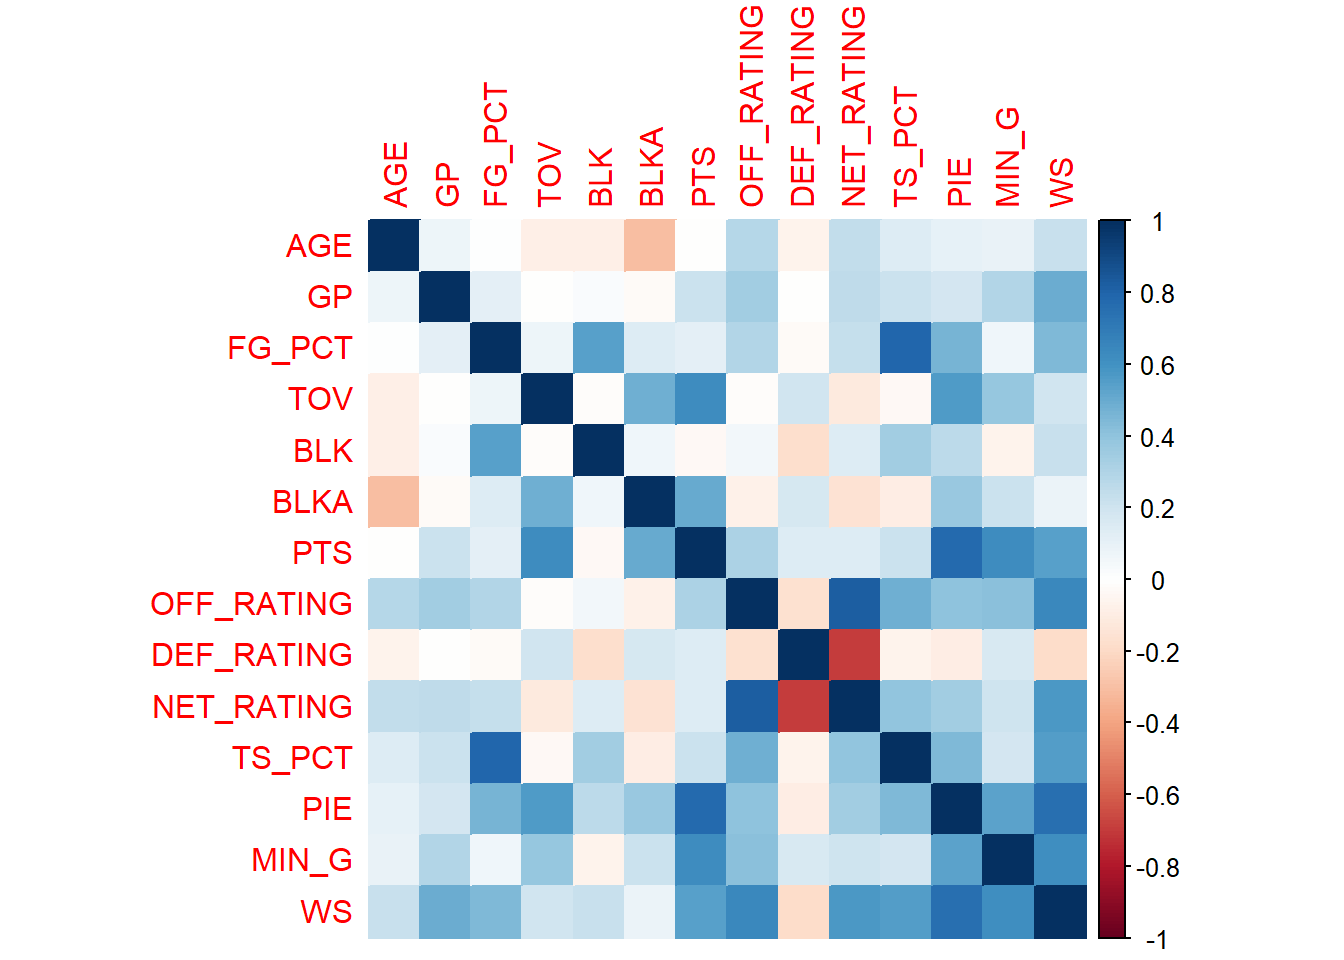
\includegraphics{Report_files/figure-latex/correlation-independent-variables-1.pdf}

There are, also in this case, different correlations between the
dependent variables.

\hypertarget{residual-analysis}{%
\paragraph{Residual analysis}\label{residual-analysis}}

\includegraphics{Report_files/figure-latex/residual-analysis-1.pdf}

From the plots the assumptions of the linear model seem to be fulfilled.
It can be seen that some players are outliers in each graph: these
players probably have special contracts (two-way contracts). This means
that they usually play in the team's second team (in a so called
development league) and occasionally in the first team, so they have
really low salaries compared to the league average.

\hypertarget{mse}{%
\paragraph{MSE}\label{mse}}

\begin{verbatim}
## [1] 4.775116e+13
\end{verbatim}

The Mean Squared Error of the reduced model is really close to the
complete model one (with the logarithmic transformation of the dependent
variable), 4.77e+13 against 4.70e+13. Considering that the complete
model has 28 variables and the reduced one 12, the latter model
represents quite an improvement.

\hypertarget{real-salaries-vs-salaries-prediction}{%
\paragraph{Real salaries vs salaries
prediction}\label{real-salaries-vs-salaries-prediction}}

\begin{verbatim}
##                      Salary Predicted salary Difference
## Bradley Beal       46741590         21945158   24796432
## Darius Garland     34005250         10821355   23183895
## Zach LaVine        40064220         17030435   23033785
## Trae Young         40064220         18771385   21292835
## Deandre Ayton      32459438         12251585   20207853
## Michael Porter Jr. 33386850         13910889   19475961
## Zion Williamson    34005250         14543954   19461296
## Karl-Anthony Towns 36016200         17724464   18291736
## Jordan Poole       27955357         10348315   17607042
## Gordon Hayward     31500000         15311898   16188102
\end{verbatim}

\begin{verbatim}
##                     Salary Predicted salary Difference
## LeBron James      47607350         79971554   32364204
## Kevin Durant      47649433         76482185   28832752
## DeMar DeRozan     28600000         51810315   23210315
## Kyrie Irving      37037037         52868441   15831404
## Nikola Vucevic    18518519         33136916   14618397
## Jalen Brunson     26346666         40868798   14522132
## Russell Westbrook  3835738         18318987   14483249
## Tyrese Maxey       4343920         18257013   13913093
## Kelly Oubre Jr.    2891467         15308000   12416533
## Brook Lopez       25000000         37263780   12263780
\end{verbatim}

Here we have a comparison between real salaries and predicted ones. The
tables contain, respectively, the most overpaid players and the most
underpaid players according to the model.

\emph{OVERPAID PLAYERS}

The most overpaid player results to be Bradley Beal. After some
brilliant seasons with Washington Wizards in which he was the league top
scorer, he signed in 2022 a maximum contract (251 million \$ in
5-years). In Washington he was the best player by far, his statlines in
the past years justify the huge contract. In 23-24 he was traded to
Phoenix (keeping the same contract) to play with Durant and Booker (two
superstars) in a team that was, on the paper, a contender for the title.
Beal, being no longer the first offensive option, had a quite different
statline compared to the previous years. Additionally, the whole Phoenix
Suns team disappointed expectations. These facts are enough to explain
that Beal 23-24 performance is not in line with his salary. Darius
Garland signed a big contract (near to the maximum) starting from 23-24
season. After showing superstar potential in 22-23, Cleveland Cavaliers
renewed his contract with an important salary increase but Garland's
performance decreased in 23-24. He is only 24, the team bet heavily on
him taking a weighted risk in order to keep with them a high potential
player. This bet didn't paid in 23-24 season. Trae Young and Zach Lavine
have superstar contracts respectively in Atlanta and Chicago, but they
are not carrying their teams as expected. Both players could be traded
during this summer. Zion Williamson and Michael Porter jr (especially
the first one) are young players that in their still short careers have
not shown their full potential due to injuries. Their contracts, let's
say, consider their potential performance at the top of their form.
Jordan Poole had an exploit in the previous seasons playing with a top
team, Golden State Warriors, that somehow justifies his salary. He
seemed to be ready to carry a team on his own, he was traded to
Washington but his first season was a failure.

\emph{UNDERPAID PLAYERS}

Lebron James and Kevin Durant are two of the best players in the league
for many years now. Even though, according to our model they should earn
much more than the maximum wage. For sure their careers and their
performance motivate a high salary, but equally surely they are not
underpaid. We think that this overestimation depends in part on the fact
that the variable AGE in the model is strongly significant, Lebron James
is 39 and Kevin Durant is 35. The same reasoning could apply to Kyrie
Irving (32) and especially Demar Derozan (34). For what concerns Nikola
Vucevic, his stats are always more than respectable. His salary is lower
than the expected probably because he seems to lack characteristics not
included in the model or generally difficult to quantify such as
defense, leadership and consistency at key moments of the season. Jalen
Brunson has shown this year that he is one of the best players in the
NBA after being somewhat underrated in the years past. We expected the
difference between his predicted and actual salary. Very similar the
situation of Tyrese Maxey, in the last year of his rookie contract. He
has shown by his performances that he is worth much more than his salary
says. Russell Westbrook is in the waning phase of his career. On the
expiry of his last superstar contract, no team in the league offered him
a comparable salary (he earned 47 millions in 2022). Consequently, he
accepted a 3.8 millions salary (veteran minimum contract) to play with
Los Angeles Clippers. For sure he is no longer a player worth 47
millions, but he is not worth 3.8 millions either. Our model interprets
pretty well the situation, stating that Westbrook should earn a 18.3
millions salary: not a superstar one, but not a minimum wage either.

Due to the presence of correlations between the independent variables,
we decided to implement models that perform well when the variables are
collinear such as Ridge regression and Lasso regression. In the next
paragraphs we want to see if the performance of these models is better
than that of the models seen so far.

\hypertarget{ridge-regression}{%
\subsubsection{Ridge regression}\label{ridge-regression}}

The subset selection methods use least squares to fit a linear model
with a subset of the predictors. Instead of controlling model complexity
by setting a subset of coefficients beta j to be zero, ridge regression
fits a model with all p predictors shrinking the coefficient estimates
towards zero. Ridge regression uses quadratic shrinking.

Lambda is a tuning parameter. In order to determine a good value of
lambda, we used cross-validation.

\includegraphics{Report_files/figure-latex/lambda-selection-1.pdf}

\begin{verbatim}
## [1] 755675.4
\end{verbatim}

\begin{verbatim}
## [1] 5.446854e+13
\end{verbatim}

In the plot above the red dotted line represents the cross-validation
curve (red dotted line) along with upper and lower standard deviation
curves along the lambda sequence (error bars). We chose the value of
lambda (755675.4) that gives minimum mean cross-validated error. The
mean squared error on the test set is 5.45e+13.

\begin{verbatim}
## 29 x 1 sparse Matrix of class "dgCMatrix"
##                        s1
## (Intercept) -34357164.687
## AGE            955164.032
## GP            -112520.427
## FG_PCT       10608799.655
## FG3_PCT      -1460374.152
## FT_PCT        -978799.822
## OREB          -211395.380
## DREB          -178163.551
## REB           -128666.930
## AST           -164552.200
## TOV            798446.003
## STL           -421067.531
## BLK            304893.669
## BLKA         -1507866.647
## PF            -176162.976
## PTS            235144.578
## OFF_RATING     105050.984
## DEF_RATING      66512.268
## NET_RATING      17276.367
## AST_TO        -877367.821
## TS_PCT      -24816362.621
## USG_PCT      25086597.182
## PIE            -60284.568
## PFD            263896.208
## MIN               886.738
## MIN_G          370677.954
## WS             967162.667
## BPM           -238067.811
## VORP          1102041.145
\end{verbatim}

\includegraphics{Report_files/figure-latex/model-with-best-lambda-1.pdf}

The final model was fitted with the best lambda on all data. The trace
plot shows how the coefficients change if lambda increases.

\begin{verbatim}
## [1] 0.6938449
\end{verbatim}

\begin{verbatim}
## [1] 4.344009e+13
\end{verbatim}

Once fitted the model on all data with the best lambda, we evaluated the
performance of the model. The 0.69 R-squared highlights a better fit
compared to the previous model (0.64) obtained after a subset selection.
Also the MSE improves, 4.34e+13 vs 4.77e+13.

The final step is the comparison between real salaries and predicted
ones.

\begin{verbatim}
##                      Salary Predicted salary Difference
## Bradley Beal       46741590         23835819   22905771
## Jordan Poole       27955357         10348317   17607040
## Klay Thompson      43219440         25696260   17523180
## Zach LaVine        40064220         22726915   17337305
## Deandre Ayton      32459438         15961704   16497734
## Darius Garland     34005250         17803526   16201724
## Michael Porter Jr. 33386850         17289756   16097094
## Tobias Harris      39270150         23308324   15961826
## Fred VanVleet      40806300         25497363   15308937
## Rudy Gobert        41000000         27551539   13448461
\end{verbatim}

\begin{verbatim}
##                     Salary Predicted salary Difference
## Tyrese Maxey       4343920         24414677   20070757
## Russell Westbrook  3835738         20700675   16864937
## Eric Gordon        3196448         19918750   16722302
## Desmond Bane       3845083         20436019   16590936
## Tyrese Haliburton  5808435         22145870   16337435
## Alperen Sengun     3536280         19253555   15717275
## Cam Thomas         2240160         17089707   14849547
## Jalen Williams     4558680         18820694   14262014
## Kelly Oubre Jr.    2891467         16543402   13651935
## Anthony Edwards   13534817         26285734   12750917
\end{verbatim}

\end{document}
